\chapter{A first look}\label{cha:first-look}

Testing the quantum nature of gravity is no easy task and many proposals seek to detect gravitationally induced entanglement between two masses \cite{Krisnanda_2020,Chevalier_2020,Pedernales_2019,Bose_2017} as a form of proof. 
For all these proposals, gravity is assumed to be mediated by a gravitational field.
During a time evolution, this field (like any other external field) can only perform local operations (LO) on the states of the test masses. If gravity is now assumed to behave classically, the propagation between the masses can be described by a classical communication (CC) channel \cite{Lami_2024,Bose_2017}.
These LOCC operations however cannot turn an initially unentangled state into an entangled one \cite{Horodecki_2009, Plenio_2005a}.
It immediately follows, that if one measures the involved masses to be entangled after a mutual gravitational interaction, gravity necessarily has to be quantum in some way.
It is important to note, that the opposite of this statement is not true. Measuring unentangled masses does not directly imply the classicality of the gravitational field.
This can be seen by considering operations that are non-LOCC and also produce unentangled states like for example the swap operation $\ket{\psi}_A\ket{\phi}_B \rightarrow \ket{\phi}_A\ket{\psi}_B$. This operations obviously can't induce entanglement to initially unentangled states, but requires the perfect exchange of quantum information between the states - which is not possible using classical communication alone.
In other words: If one prepares masses initially in a pure product state and measures \textit{any} state which cannot be obtained by LOCC-operations after some final time evolution, it is impossible for gravity to behave classical. One can even go so far and define the term \emph{quantum gravity} as any interaction mediated by gravity that cannot be described by LOCC operations alone \cite{Lami_2024}.

A plausible and logical idea for an experiment to test for gravitational induced entanglement is described in this chapter - which is, as a reminder, enough to prove a quantum nature of gravity.
It requires the generation of coherent delocalized quantum superpositions of massive objects either as so-called Schrödinger-cat states or squeezed gaussian states \cite{Bose_2017, Pedernales_2023}. Theses masses are brought close enough together for gravity to have a measurable effect. The distances between different parts of the spatial superpositions must have different distances to the delocalized second mass. As a result - and of course \textit{if gravity behaves quantum} - the states should get entangled.
To see this, consider the ideal simplification of a real experimental setup where two bodies with mass $m$ are trapped in an harmonic potential well (like for example an levitated particle in an optical or magnetic trap) with frequency $\omega$ separated by a distance $d$. The local Hamiltonian of the system is given by
\begin{equation}
  \op{H}_0 = \sum_{i = 1,2} \frac{\op{p}_i^2}{2m} + \frac{1}{2}m\omega^2\op{x}^2_i
\end{equation}
where $\op{x}$ and $\op{p}$ are the position and momentum operators satisfying the canonical commutation relation $[\op{x}_i, \op{p}_j] = i\hbar \delta_{ij}$.
For now, all non-gravitational interactions between the masses have been ignored. 
In the low energy regime, where the energy transfer during a process is far below the Planck scale $m_p c^2 \sim 10^{19}\si{GeV}$, gravity can be traded as an effective field theory with tools available similar to those for the electromagnetic field and QED \cite{Carney_2018}. 
In the non-relativistic limit $v \ll c$, the gravitational interaction can be described by a Newtonian $1/r$ potential acting on the center-of-mass positions, with all classical quantities are replaced by quantum operators \cite{Carney_2018,Pedernales_2023,Christodoulou_2022}. 
Spatial superpositions lead to superpositions of the metric and consequently (in the non-relativistic limit) to a superposed Newtonian potential.
The interaction Hamiltonian $\op{H}_G$ should therefore be describable by
\begin{equation}\label{eq:2:gravity-hamiltonian}
  \op{H}_G = - \frac{Gm^2}{\abs{d - \op{x}_1 + \op{x}_2}} ,
\end{equation}
where $G=6.6743 \times 10^{-11} \si{m^3 kg^{-1} s^{-2}}$ is the gravitational constant. The separation of the masses $d$ is chosen much larger than the extension of the delocalization (in this setup comparable to the position variance of the harmonic oscillator). This condition is realistic given that the biggest spatial delocalization ever achieved in matter wave experiments is in the order of $500\si{nm}$ \cite{Fein_2019}.
Expanding the Hamiltonian $\op{H}_G$ for small $\op{x}_i$, only the second order term proportional to $(\op{x}_1 - \op{x}_2)^2$ can induce entanglement \cite{Krisnanda_2020}. The zeroth order term is just a overall energy offset, the first order term $\propto (\op{x}_1 - \op{x}_2)$ as well as the terms $\op{x}^2_i$ result only in a local interaction for each mass separately. The coupling term $ - (\op{x}_1\op{x}_2 + \op{x}_2\op{x}_1) = -2\op{x}_1\op{x}_2$ however is very interesting as it couples both oscillators and can thus mediate entanglement.
Introducing the ladder operators, the Hamiltonian $\op{H}=\op{H}_0 + \op{H}_G$ can be expressed as \cite{Carney_2018}:
\begin{equation}\label{eq:2:general-hamiltonian}
  \op{H} = \sum_{i=1,2} \hbar \omega \op{a}_i^\dagger \op{a}_i - \frac{Gm^2}{d^3} \left(\sqrt{\frac{\hbar}{2m\omega}}\right)^2 \left( \op{a}_1\op{a}_2 + \op{a}_1\op{a}^\dagger_2 + \op{a}^\dagger_1\op{a}_2 + \op{a}^\dagger_1\op{a}^\dagger_2 \right)
\end{equation}
Applying the \textit{rotating-wave approximation}\footnote{This approximation is known from quantum optics, where all fast oscillating terms in the Hamiltonian can be dropped \cite{Carney_2018,Lami_2024}. In the interaction picture, the ladder operators evolve as $\op{a}(t) = \op{a}e^{-i\omega t}$. The terms like $\op{a}_1(t)\op{a}_2(t)$ oscillate with frequency $2\omega$ whereas $\op{a}_1^\dagger(t) \op{a}_2(t)$ does not oscillate at all. Due to the small coupling, this approximation works very well here.}, the terms $\op{a}_1\op{a}_2 + \op{a}^\dagger_1\op{a}^\dagger_2$ can be dropped. Defining the coupling strength $g$ of the interaction as $g = Gm/\omega d^3$, eq \eqref{eq:2:general-hamiltonian} can be rewritten as
\begin{equation}
  \op{H} = \sum_{i=1,2} \hbar \omega \op{a}_i^\dagger \op{a}_i - \hbar g \left( \op{a}_1\op{a}^\dagger_2 + \op{a}^\dagger_1\op{a}_2 \right) .
\end{equation}
Now, for simplicity and as a simple example, the evolution of the initial Fock state $\ket{\psi(0)} = \ket{10}$ is considered. The gravitational interaction $H_G$ can be treated as a time dependent perturbation and the state evolution is given as (for calculation see appendix \ref{apx:general-state-perturbation-theory}) \cite{Carney_2018}
\begin{equation} \label{eq:2:general-evolved-state}
  \ket{\psi(t = 0)} = \ket{10} \xrightarrow{\text{time }t} \ket{\psi(t)} =  \mathcal{N} \left(\ket{10} - i g t \ket{01} + \mathcal{O}(g^2) \right)
\end{equation}
where $\mathcal{N}$ is an appropriate normalization constant. The evolved state \eqref{eq:2:general-evolved-state} is entangled and cannot be reduced into a product of two oscillator Fock states. The entanglement is very small since it is proportional to the gravitational coupling constant $gt$ \footnote{The amount of entanglement can for example be quantified with the later introduced \textit{logarithmic negativity} $E_N$. For this state, it is given by $E_N(\ketbra{\psi(t)}) \simeq 2tg/\log 2 + \mathcal{O}(g^2) \geq 0$.}.
Another interesting result, which underlines the false inference of a classical gravity from observed non-entanglement discussed above can be seen by considering the time evolution of a coherent product state $\ket{\alpha} \otimes \ket{\beta}$ where $\op{a}\ket{\alpha} = \alpha\ket{\alpha}$. The time evolution is derived in appendix \ref{apx:general-coherent-state-evolution} and results in
\begin{equation}
  e^{-i\op{H}t/\hbar} \left( \ket{\alpha} \otimes \ket{\beta} \right) = \ket{ e^{-i\omega t} \left( \alpha \cos gt - \beta \sin gt \right) }\otimes\ket{ e^{-i\omega t} \left( - \alpha \sin gt + \beta \cos gt \right) } .
\end{equation}
This state is clearly a product state and thus not entangled. But for a time $t_0 = \pi/2g$ the state is effectively the swapped initial state $\ket{\beta} \otimes \ket{\alpha}$ up to a local phase. This swap operation is however, as established earlier, not possible under a LOCC protocol. Thus, even if the resulting state after time evolution under a gravitational interaction is unentangled, we can role out the classicality of gravity \cite{Carney_2018,Lami_2024}. 
Gravity must therefore be capable of transmitting quantum information and must be described by a quantum channel.

Experimentally, one requires the ability to generate spatial superpositions of two massive objects with large enough coherence times. Usually the weak gravitational interaction requires coherence times in the order of $100\si{ms} - 10\si{s}$ for any meaningful and measurable entanglement to built up. The masses should additionally be massive enough for their gravitational effects to be measurable.
These requirements impose huge experimental and engineering challenges. To contextualize: The most massive object ever put into a spatial superposition in matter-wave interferometry is in the order of $4 \times 10^{-23}\si{kg}$ \cite{Fein_2019}, whereas the smallest object whose gravitational field has been measured was just below $100 \si{mg}$ \cite{Westphal_2021} - a difference of $19$ orders of magnitude.
One way to experimentally create such spatial superpositions is giving the masses a spin-1/2 degree of freedom. For example, a nitrogen-vacancy diamonds can be used \cite{Bose_2017}, where the NV site provides the required spin of 1/2. An applied magnetic gradient $\partial_x B$ functions like a \q{beam splitter} and creates a delocalized state.
The extend of this superposition can be calculated and separations in the order of $100 \si{\mu m}$ are theoretically achievable \cite{Bose_2017}.
Levitated, trapped particles isolated and shielded in a vacuum can increase environmental isolation by avoiding contact with surrounding noise. The additional forces due to the trapping potential or the gravitational acceleration can be studied in advance. 
In this thesis, I assume that all required states and superpositions can be prepared experimentally.

The general and idealized problem considered is illustrated in \cref{fig:2:simple-problem}.
\begin{figure}[!htbp]
  \centering
  \def\svgwidth{\textwidth}
  \input{./../figures/simple-problem.pdf_tex}
  \caption{Schematic figure of the proposed experiment with two masses prepared in a spatial superposition state. The gravitational interaction $\op{H}$ induces different phases to each of the superpositions due to the different distances between all masses. This results in measurable entanglement after some time evolution.}
  \label{fig:2:simple-problem}
\end{figure}
Two massive bodies with masses $M_A$ and $M_B$ are initially separated by a center-to-center distance $2L$. The masses are prepared in a coherent delocalized quantum superposition Schrödinger-cat-like state in, for now, a parallel orientation as depicted in \cref{fig:2:simple-problem}.
The extension of the superposition is denoted by $\Delta x$ and is the same for both masses.
It is important to choose the positions of the masses such that the distances between each part of the delocalized mass $A$ and $B$ are not always identical. 
Otherwise, all built up phases are the same and no entanglement is observable.
With the notation introduced in \cref{fig:2:simple-problem}, the initial state at $t=0$ is given by
\begin{equation}\label{eq:2:initial-state}
  \ket{\psi(t=0)} = \frac{1}{2}\left( \ket{\psi_A^1} + \ket{\psi_A^2} \right) \otimes \left( \ket{\psi_B^1} + \ket{\psi_B^2} \right) .
\end{equation}
The state evolves under a Hamiltonian $\op{H}$ and after some time the position of each mass is measured and checked for entanglement.
For now I assume that all interactions except gravity can be neglected. In reality, electromagnetic forces and Casimir-Polder interactions \cite{Casimir_1948, Casimir_1948a} need to be considered.

As established earlier in this chapter, with some assumptions made, gravitational interaction can generate entanglement. In the time scales of the experiment, the acceleration of the masses due to the mutual gravitational interaction can be neglected \footnote{Take for example a silica sphere ($\rho = 2648 \si{kg/m^3}$) with $R=10^{-5}\si{m}$ separated by $2L=4R$. The mutual gravitational acceleration for each sphere is around $a=GM/(2L)^2 = 5 \times 10^{-13}\si{m/s^2}$ which results for $t\sim 1 \si{s}$ in a distance traveled of $\sim 10^{-13}\si{m}$.}. The Hamiltonian therefore only needs to include the gravitational potential 
\begin{equation} \label{eq:2:potential}
  \op{V} = -\frac{GM_AM_B}{\abs{\op{D}}}
\end{equation}
where $\op{D}$ is the distance operator between the masses. It depends on the individual positions $\op{x}_A$ and $\op{x}_B$.
During time evolution, the different parts of the superpositions built up different local phases. I am interested in calculating, how much entanglement one can expect from this kind of interactions.


\section{Time evolution under a gravitational potential}\label{sec:2:time-evolution}

The time evolution of a quantum system is governed by the Schrödinger-equation
\begin{equation}
  i\hbar \pdv{t} \ket{\psi(t)} = \op{H} \ket{\psi(t)}
\end{equation}
where in this case the interaction Hamiltonian responsible for the entanglement dynamics is given by $\op{H} = \op{V}$ in eq. \eqref{eq:2:newtonian-potential}.
The eigenbasis of $\op{V}$ is given by $\left\{ \ket{\psi_A^{(1)}}, \ket{\psi_A^{(2)}} \right\}\otimes \left\{ \ket{\psi_B^{(1)}}, \ket{\psi_B^{(2)}} \right\}$, as all these states are eigenstates of the distance operator $\op{L}$
\begin{equation}
  \op{V} \ket{\psi^{(i)}_A} \otimes \ket{\psi^{(j)}_B} = -\frac{G M_A M_B}{2L^{(ij)}} \ket{\psi^{(i)}_A} \otimes \ket{\psi^{(j)}_B} .
\end{equation}
The Schrödinger equation for the diagonal Hamiltonian $\op{H}$ can be directly solved for the initial state eq. \eqref{eq:2:initial-state} with the solution given by 
\begin{equation}
  \ket{\psi(t)} = \frac{1}{2} \sum_{i,j\in\{1,2\}} \exp{\frac{i}{\hbar} \frac{G M_A M_B}{2L^{(ij)}} t} \ket{\psi^{(i)}_A \psi^{(j)}_B}
\end{equation}
where the tensor product $\otimes$ was omitted.
It is possible to express the state using the dynamically accumulated phases $\phi^{(ij)}$ which build-up after a mutual interaction as
\begin{equation}\label{eq:2:evolved-state}
  \ket{\psi(t)} = \frac{1}{2}\bigl(
    e^{i\phi^{(11)}} \ket{\psi_A^{(1)} \psi_B^{(1)}} 
    + e^{i\phi^{(12)}} \ket{\psi_A^{(1)} \psi_B^{(2)}}
    + e^{i\phi^{(21)}} \ket{\psi_A^{(2)} \psi_B^{(1)}} 
    + e^{i\phi^{(22)}} \ket{\psi_A^{(2)} \psi_B^{(2)}} \bigr) .
\end{equation}
The phases $\phi^{(ij)}$ in the specific setup shown in \cref{fig:2:simple-problem} are given by
\begin{align}
  \phi \equiv \phi^{(11)} = \phi^{(22)} = \frac{G M_A M_B}{2\hbar L}t 
  \qquad \text{and} \qquad 
  \phi^{(12)} = \phi^{(21)} = \frac{G M_A M_B}{\hbar \sqrt{4L^2 + (\Delta x)^2}}t ,
\end{align}
By expanding the phases for small superposition sizes $\Delta x \ll L$, the global phase $\phi$ can be factored out of the evolved state
\begin{equation}\label{eq:2:definition-delta-phi}
  \phi^{(12)} = \phi^{(21)} \approx \frac{GM_AM_B}{\hbar} \left[ \frac{1}{2L} - \frac{(\Delta x)^2}{16 L^3} \right] t \equiv \phi - \Delta\phi .
\end{equation}
which ultimately can be written in the form
\begin{equation}\label{eq:2:evolved-state-factored}
  \ket{\psi(t)} = e^{i\phi}\frac{1}{\sqrt{2}}\left[ 
    \ket{\psi_A^{(1)}} \otimes \frac{\ket{\psi_B^{(1)}} + e^{-i\Delta\phi} \ket{\psi_B^{(2)}}}{\sqrt{2}}
    + \ket{\psi_A^{(2)}} \otimes \frac{e^{-i\Delta\phi} \ket{\psi_B^{(1)}} + \ket{\psi_B^{(2)}}}{\sqrt{2}} \right] .
\end{equation}
One can see immediately that in general, the resulting state cannot be written as a product state, hence it is entangled.
This is of course only the case, if $\Delta \phi \neq k\pi$ with integer $k\in \mathbb{N}$.

In order to assess quantitatively how entangled the state $\ket{\psi(t)}$ is after time $t$, a more sophisticated measure is required. 
One possible measure is the \q{logarithmic negativity}, which is introduced in the next section and used in the rest of this work.

\section{Entanglement measures}\label{sec:2:entanglement-measures}
Checking whether an arbitrary state $\rho$ is entangled or not is no easy task. In fact, this problem is known to be NP-hard \cite{Gurvits_2003}.
A state $\rho_{AB} \in \mathcal{H}_A\otimes\mathcal{H}_B$ is called entangled, if it is \emph{non-separable}, that is, it cannot be expressed as a tensor product of two subsystems $\rho_A \in \mathcal{H}_A$ and $\rho_B \in \mathcal{H}_B$.
Only for specific cases - like the case of two qubits or qubit-qutrit - a simple sufficient criterion for determining the separability of a general mixed state is known:
The positive partial transpose (PPT) criterion states, that if the partial transpose of the density matrix is positive ($\rho^{\Gamma_A} > 0$ \footnote{A matrix is defined as positive (\q{positive definite}), if all eigenvalues are positive.}), the state $\rho$ is separable \cite{Horodecki_2009,Plenio_2005a}.
In other words, if $\rho^{\Gamma_A}$ has negative eigenvalues, $\rho$ is guaranteed to describe an entangled state.
The inverse is true, if and only if the dimension of $\rho_A\otimes\rho_B$ is $2\times2$ or $3\times2$ \cite{Horodecki_2009} - otherwise, only having non-negative eigenvalues doesn't necessarily result in an unentangled system.
The partial transpose with respect to a subsystem $i$ can be understood in the same way as the partial trace, where the operation (in this case the transform) is performed only on indices corresponding the subsystem $\rho_i$.
It is defined for an arbitrary density operator $\rho = \sum_{ijkl}p^{ij}_{kl}\ketbra{i}{j}\otimes\ketbra{k}{l}$ as $\rho^{\Gamma_A} = \sum_{ijkl}p^{ji}_{kl}\ketbra{i}{j}\otimes\ketbra{k}{l}$.
To see the necessity of the PPT criterion, consider a separable mixed state $\rho$, which can be generally expressed as 
\begin{equation}\label{eq:2:separable-state}
  \rho = \sum p_i \rho_{A}^{(i)}\otimes\rho_{B}^{(i)} .
\end{equation}
The partial transpose is in this case trivial:
\begin{equation}
  \rho^{\Gamma_A} = \sum p_i (\rho_{A}^{(i)})^T \otimes \rho_{B}^{(i)} .
\end{equation}
Since the transpose preserves eigenvalues, the transposed subsystem $A$ is still positive $(\rho_{A}^{(i)})^T > 0$ and describes again a valid quantum state. It follows, that $\rho^{\Gamma_A}$ is positive as well.
If somehow $\rho^{\Gamma_A}$ has any negative eigenvalues, this can only mean that the initial state $\rho$ is not separable and cannot be expressed in the form of eq. \eqref{eq:2:separable-state} and the necessity of the criterion is shown.

For quantifying entanglement in a more precise way, a mathematical quantity called \emph{entanglement measure} can be used. A good measure should be able to capture the essential features of entanglement. One can axiomatically state what properties such a measure $E(\rho)$ should have \cite{Plenio_2005a,Horodecki_2009}:
\begin{description}
  \item[Normalization] An entanglement measure should be a map from a state to a positive real number:
  \begin{equation}
    \rho \rightarrow E(\rho) \in \mathbb{R}^+
  \end{equation}
  where usually the maximally entangled state has $E=1$.
  \item[Monotonicity under LOCC] $E$ should not increase under local operations and classical communications. This is the most important postulate for an entanglement measure and often cited as the \textit{only} required postulate.
  \item[Vanishing on separable states] $E(\rho)=0$ if $\rho$ is separable
  \item[] Often one finds additional properties useful like \textit{convexity} $E(\sum p_i \rho_i) \leq \sum p_i E(\rho_i)$ or (full) \textit{additivity} $E(\rho \otimes \sigma) = E(\rho) + E(\sigma)$.
\end{description}
A function that satisfies these conditions is often called an \textit{entanglement monotone}.

The \emph{negativity} $\mathcal{N}$ is such an entanglement monotone \cite{Vidal_2001,Plenio_2005a} that used the PPT criterion to determine if a state is entangled or not. It is defined as 
\begin{equation}\label{eq:2:negativity}
  \mathcal{N} = \frac{\norm{\rho^{\Gamma_A}}_1 - 1}{2}
\end{equation}
where $\norm{A}_1 = \tr\abs{A} = \tr \sqrt{A^\dagger A}$ is the trace norm. The negativity however is not additive and a more universally applicable and widely used entanglement measure is the \emph{logarithmic negativity} \cite{Plenio_2005}
\begin{equation}\label{eq:2:logarithmic-negativity}
  E_N(\rho) = \log_2\norm{\rho^{\Gamma_A}}_1 .
\end{equation}
The monotonicity of the logarithm implies that $E_N$ is an entanglement monotone as well.
Furthermore, it is noteworthy, that $\norm{\rho^{\Gamma_A}} = \norm{\rho^{\Gamma_B}}$ as will be shown below. Therefore, the logarithmic negativity is symmetric under exchange of to the subsystem.

\begin{proposition}
  a) The partial transpose w.r.t. subsystem $A$ is equal to the transposed partial transpose w.r.t. subsystem $B$: $\rho^{\Gamma_A} = (\rho^{\Gamma_B})^T$. 
  b) The trace norms of partially transposed density operators w.r.t. any subsystem are equal: $\norm{\rho^{\Gamma_A}}_1 = \norm{\rho^{\Gamma_B}}_1$.
\end{proposition}
\begin{proof}
  a) A general density matrix $\rho$ can be expressed as
  \begin{equation*}
    \rho = \sum_{i,j,k,l} \rho_{ij,kl} \ketbra{i}{j}_A\otimes\ketbra{k}{l}_B
  \end{equation*}
  The partial transpose with respect to subsystem $B$ is then defined as 
  \begin{equation*}
    \rho^{\Gamma_B} \equiv \sum_{i,j,k,l} \rho_{ij,kl} \ketbra{i}{j}_A\otimes\left(\ketbra{k}{l}_B\right)^T = \sum_{i,j,k,l} c_{ij,kl} \ketbra{i}{j}_A\otimes\ketbra{l}{k}_B
  \end{equation*}
  The complete transpose of this is
  \begin{equation*}
    (\rho^{\Gamma_B})^T = \sum_{i,j,k,l} \rho_{ij,kl} \left(\ketbra{i}{j}_A\right)^T\otimes\left(\ketbra{l}{k}_B\right)^T = \sum_{i,j,k,l} c_{ij,kl} \ketbra{j}{i}_A\otimes\ketbra{k}{l}_B \equiv \rho^{\Gamma_A}
  \end{equation*}
  b) Clear by a) and by using \cref{lemma:trace-norm-hermitian} and the fact that the eigenvalues of a square matrix $A$ and $A^T$ are equal.
\end{proof}

The logarithmic negativity is very easy to calculate compared to other entanglement measures.
If the eigenvalues of $\rho$ are known, the logarithmic negativity can be directly computed, as will be demonstrated below. Since this thesis focuses on low-dimensional $4 \times 4$ systems, single eigenvalues can be determined with low effort analytically as well as numerically with great stability.

\begin{lemma}\label{lemma:trace-norm-hermitian}
  The trace norm $\norm{A}_1 \equiv \tr \sqrt{A^\dagger A}$ of a hermitian matrix $A$ is equal to the sum of the absolute eigenvalues of $A$.
\end{lemma}
\begin{proof}
  This can be immediately seen by the spectral decomposition $\operatorname{\lambda}(A) = \{\lambda_1,...\}$:
  \begin{equation*}
    \tr \sqrt{A^\dagger A} = \tr \sqrt{A^2} = \tr{U\sqrt{\diag(\lambda_1, \dots)^2}U^\dagger} = \sum_i \sqrt{\lambda_i^2} = \sum_i \abs{\lambda_i}.
  \end{equation*}
\end{proof}

\begin{proposition}\label{proposition:negativity}
  The negativity eq. \eqref{eq:2:negativity} is given as the absolute sum of all negative eigenvalues of $\rho^{\Gamma}$: 
\begin{equation}
    \mathscr{N}(\rho) \equiv \frac{\norm{\rho^{\Gamma}}_1 - 1}{2} = \abs{\sum_{\lambda_i < 0} \lambda_i}.
\end{equation}
\end{proposition}
\begin{proof}
  The proof is in parts given by Vidal and Werner \cite{Vidal_2001}. It is known that the density matrix is hermitian: $\rho = \rho^\dagger$. Using \cref{lemma:trace-norm-hermitian}, the trace norm of the density matrix is given as $\norm{\rho}_1=\sum \lambda_i = \tr \rho = 1$. The partial transpose $\rho^{\Gamma}$ obviously also satisfies $\tr \rho^{\Gamma} = 1$ but might have negative eigenvalues. Since $\rho^{\Gamma}$ is still hermitian, the trace norm is given by
  \begin{equation*}
    \norm{\rho^{\Gamma}}_1 = \sum_i\abs{\lambda_i} = \sum_{\lambda_i \ge 0} \lambda_i + \sum_{\lambda_i < 0} \abs{\lambda_i} = \sum_i \lambda_i + 2\sum_{\lambda_i < 0} \abs{\lambda_i} = 1 + 2\sum_{\lambda_i < 0} \abs{\lambda_i} ,
  \end{equation*}
  where in the last step $\sum \lambda_i = \tr \rho^{\Gamma} = 1$ was used.
\end{proof}
\begin{remark}
  The PPT criterion states, that if $\rho^{\Gamma}$ has negative eigenvalues, the state $\rho$ is entangled. The negativity uses this criterion for a quantification of entanglement. This motivates the name \textit{negativ}ity.
\end{remark}

Calculating the logarithmic negativity of the evolved state eq. \eqref{eq:2:evolved-state}, it is possible to quantify how the entanglement behaves in time. A straight forward computation following the calculation methods established above yields (for detailed calculations see appendix \ref{apx:E_N-exemplary})
\begin{equation}\label{eq:2:entanglement-dynamics-parallel}
  E_N(\ketbra{\psi(t)}) = \log_2\left(1 + \abs{\sin \Delta\phi}\right) .
\end{equation}
As expected, the states are not entangled for $\Delta\phi = k\pi, \ k\in\mathbb{Z}$ and maximum entanglement $E_N = 1$  is reached
for $\Delta\phi = 2\pi k \pm \pi/2$.
This result aligns with the previous observations by
demanding that the evolved state eq. \eqref{eq:2:evolved-state-factored}  is separable.
The complete entanglement dynamics are shown in \cref{fig:2:entanglement-dynamics}.
\begin{figure}[!htbp]
  \centering
  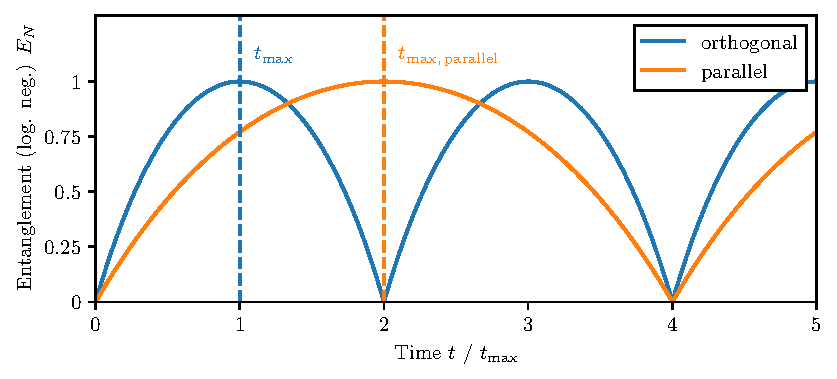
\includegraphics[width=\textwidth]{./../figures/ideal-entanglement/EN-time.pdf}
  \caption{Entanglement dynamics quantified by the logarithmic negativity $E_N$ for two different orientations of the spatial superpositions. The parallel orientation (\textbf{orange}) is shown in \cref{fig:2:simple-problem} and the orthogonal orientation (\textbf{blue}) was taken from Ref. \cite{Pedernales_2023}, where the cat-states are right-angled compared to the parallel configuration. The maximal amount of entanglement is reached after a time given by eq. \eqref{eq:2:t-max-parallel} and for reasonable parameters this equates to $t_\mathrm{max,\,orthogonal} \equiv t_\mathrm{max} \approx 129\si{ms}$.}
  \label{fig:2:entanglement-dynamics}
\end{figure}
Additionally, this figure depicts the entanglement generation in the \q{orthogonal orientation}, where both superpositions are aligned in a straight line right-angled to the previously used setup in \cref{fig:2:simple-problem}.

The time $t_\mathrm{max,\,parallel}$ at which the states are maximally entangled for the first time, can be calculated by using the definition of $\Delta\phi$ from eq. \eqref{eq:2:definition-delta-phi} as
\begin{equation}\label{eq:2:t-max-parallel}
  t_\mathrm{max,\,parallel} = \frac{8 \pi L^3\hbar}{G M_A M_B (\Delta x)^2} .
\end{equation}
In the orthogonal orientation, this point in time is reached twice as fast \cite{Pedernales_2023}. This is because in this orientation, the difference in distances between the cat-states is maximized and consequently the relative dynamical phase build-up is faster compared to the parallel orientation resulting in a faster entanglement rate.

This suggests, that the orthogonal orientation might be beneficial as it requires shorter coherence times. This effect is studied in more detail in \cref{sec:4:optimal-setup}.
To give an estimation of the coherence times needed, consider two identical silica nano-spheres with densities $\rho=2648\si{kg/m^3}$ and radii $R=10^{-5}\si{m}=10\si{\mu m}$ separated by a distance $2L = 4R$.
The superposition size is in the order of $100\si{nm}$.
The maximum entanglement in the parallel configuration is reached after a time $t_\mathrm{max,\,parallel} \approx 258\si{ms}$ which is quite long and challenging experimentally considering that possible coherence times are currently only in the order of micro-seconds \cite{OConnell_2010}.


\section{Issues with the idealized experimental procedure}\label{sec:2:experimental-problems}

For the practical realization of an experiment on measuring gravitationally induced entanglement of masses, other forms of direct or indirect interaction between the particles must be suppressed such that the measured entanglement ultimately arises only due to their gravitational interaction.
In particular, the short-range \emph{Casimir interactions} \cite{Casimir_1948} discussed in \cref{cha:casimir-effect} have to be shielded as they exert a much greater attraction force on the particles at small separations than gravity.
It is still a hot topic of discussions whether Casimir interactions can even entangle macroscopic bodies at all, as it is not even clear if it is a conservative force in the first place - although most researchers believe it is \cite{DeBiase_2012,Yi_2023}.
To estimate the minimal particle-particle separation $2L$ while requiring that the gravitational interaction $V_\mathrm{Gravity}$ is stronger than the Casimir interactions $V_\mathrm{Casimir}$ \cite{Emig_2007} by a factor $\chi > 1$, the following inequality can be stated:
\begin{align}
  \chi \abs{V_\mathrm{Casimir}} &\leq \abs{V_\mathrm{Gravity}} \\
  \Longleftrightarrow \quad \chi \frac{23 \hbar c}{4 \pi (2L)^7} \left(\frac{\varepsilon_r - 1}{\varepsilon_r + 2}\right)^2 R^6 &\leq  \frac{G M^2}{2L} .\qquad\qquad\qquad\qquad
\end{align}
Using $M = 4/3 \pi R^3\rho_\mathrm{Silica}$, the minimum separation distance is independent of the size of the particle and is given by
\begin{equation}
  L \geq \left(\frac{207}{4096} \frac{\hbar c}{\pi^3 G \rho_\mathrm{Silica}^2}\right)^{1/6} \sqrt[6]{\chi} \approx 69\si{\mu m} \sqrt[6]{\chi} .
\end{equation}
For the same particle as used before, the time for a single measurement, i.e. the coherence time $t_\mathrm{max} \approx 30\si{s} \sqrt{\chi}$ is very large.
The field of levitated particles is promising for these experiments as it offers an isolated, noise-reduced environment while still allowing for exceptional force sensitivity as well as precise quantum control and thus long coherence times \cite{Aspelmeyer_2024,GonzalezBallestero_2021}.
Nevertheless, it would be beneficial to reduce the separation distance between the particles for a shorter measurement time.
For this, usually a conducting \emph{Faraday shield} between the particles is proposed \cite{Kamp_2020}.
Such a shield would simultaneously suppress all other forms of electromagnetic interactions such as Coulomb forces, if the particles happened to be charged.
Coulomb forces have the ability to entangle the particles as well\footnote{In fact, the Aspelmeyer group is currently working on an experiment trying to measure entanglement due to Coulomb interactions \cite{Rudolph_2022}.} and due to the similar distance behavior for Coulomb and gravitational interactions as well as the stronger coupling, these interactions could potentially be problematic.

This thesis is focused around the problems which arise in the generation of entanglement in the presence of the Faraday shield.
Reconstructing the position states of the masses requires many experimental runs and small variations in the initial setup between measurements introduce effective decoherence.
Casimir interactions between the particles and the newly placed Faraday shield can ultimately destroy entanglement in the final averaged measurement.
In \cref{cha:entanglement-generation} this effect is analyzed in depth, narrowing the range of viable parameters for particle-shield separation, superposition size, and particle mass.
Additionally, thermal vibrations and shield-induced noise are explored in \cref{cha:the-shield}.
